% IEEE journal version of the manuscript.
% Build: pdflatex main && bibtex main && pdflatex main && pdflatex main   (or upload the paper/ folder to Overleaf)
% Items marked in red (\todo) must be completed before submission.
% Figures 1, 3 and 5 are produced by tools/make_paper_figures.py; once the PNGs are copied into
% paper/figures/ they replace the placeholder boxes automatically.
\documentclass[journal]{IEEEtran}

\usepackage[T1]{fontenc}
\usepackage{amsmath,amssymb}
\usepackage{graphicx}
\usepackage{booktabs}
\usepackage{array}
\usepackage{cite}
\usepackage{url}
\usepackage{xcolor}
\usepackage[hidelinks]{hyperref}

\graphicspath{{figures/}}
\newcommand{\todo}[1]{\textcolor{red}{[#1]}}
\newcommand{\figorplaceholder}[3]{%
  \IfFileExists{figures/#1}%
    {\includegraphics[width=#3]{#1}}%
    {\framebox[#3]{\parbox[c][#2][c]{0.9#3}{\centering
      {\small\color{red}\itshape Placeholder: insert figures/\detokenize{#1}\par}
      \vspace{2pt}{\footnotesize generated by tools/make\_paper\_figures.py (see paper/README.md)\par}}}}}
\newcommand{\fname}[1]{\texttt{#1}}
\newcommand{\R}{\mathbb{R}}

\hyphenation{Efficient-Net Transformer-Conv Py-Torch}

\begin{document}

\title{Uncertainty-Gated Fusion of EfficientNet-B3 and a Multi-Scale Graph Pyramid for Four-Class Brain Tumour MRI Classification: An Audited Cross-Validation Study}

\author{\todo{First Author},~\todo{Second Author},~and~\todo{Supervisor Name}%
\thanks{\todo{Authors} are with the \todo{Department}, \todo{Institution}, \todo{City}, \todo{Country} (e-mail: \todo{corresponding author e-mail}).}%
\thanks{Funding: \todo{to be completed}. The authors declare no competing interests \todo{confirm}.}}

\markboth{\todo{Journal name}}{\todo{Author} \MakeLowercase{\textit{et al.}}: Uncertainty-Gated EfficientNet--Graph Fusion for Brain Tumour MRI}

\maketitle

\begin{abstract}
Deep networks often report near-perfect accuracy on public brain tumour MRI collections, yet calibration and the effect of duplicated images are rarely examined. We propose a dual-stream classifier that pairs an ImageNet-pretrained EfficientNet-B3 with a three-level graph pyramid of 336 regional nodes processed by parallel GCN, GAT and TransformerConv paths. The two 384-dimensional embeddings are refined by dynamic recalibration and a two-token cross-modal transformer, and fused by a gate driven by Monte Carlo (MC) dropout uncertainty. The model (19.35\,M parameters) was evaluated on a public four-class dataset of 12,064 contrast-enhanced T1-weighted images with image-level stratified five-fold cross-validation and ten-view test-time augmentation, and every metric was recomputed from the saved per-image out-of-fold predictions. Accuracy was $99.15 \pm 0.39\%$ (range 98.47--99.46\%) and macro-F1 $99.15 \pm 0.40\%$; pooled accuracy was 99.15\% (95\% bootstrap CI 98.99--99.31\%). Class-wise sensitivity ranged from 98.53\% to 99.58\% and specificity was at least 99.68\%; only 0.20\% of tumour images were classified as tumour-free. The expected calibration error was $0.021 \pm 0.003$, reflecting mild under-confidence attributable to label smoothing. A file-level audit showed that 35.2\% of the images are offline-augmented copies of 620 source slices, almost all with a sibling in the training partition, yet their accuracy (99.15\%) matched that of the remaining images (99.14\%). Because patient identifiers are unavailable and cross-source near-duplicates cannot be excluded, these are image-level estimates; duplicate-aware validation, component ablations and external testing are required before claims of generalisation.
\end{abstract}

\begin{IEEEkeywords}
Brain tumour classification, magnetic resonance imaging, graph neural networks, EfficientNet, multimodal fusion, Monte Carlo dropout, calibration, data leakage, cross-validation.
\end{IEEEkeywords}

% =====================================================================
\section{Introduction}
\IEEEPARstart{G}{liomas}, meningiomas and pituitary tumours differ in origin, treatment and prognosis, and their distinction on MRI shapes the first clinical decisions~\cite{louis2021who}. Contrast-enhanced T1-weighted images form the basis of the most widely used public datasets for this task~\cite{cheng2015enhanced}. Automated classification of these tumour types, with or without a tumour-free class, is a widely studied triage and second-reader task~\cite{cheng2015enhanced,deepak2019brain,swati2019brain,badza2020classification,tummala2022classification}.

Convolutional neural networks (CNNs) with transfer learning dominate this task and typically report accuracies in the mid- to high-90 percent range on public collections~\cite{deepak2019brain,swati2019brain,badza2020classification}. Vision transformers report similar figures~\cite{tummala2022classification}. Two properties of these models remain under-examined. First, a CNN pools local evidence into one global vector, so explicit relations between distant regions are learned only implicitly. Graph formulations make such relations explicit, and hybrid CNN--graph models have recently been applied to brain tumour MRI~\cite{gursoy2024braingcn}. Second, most systems output a single softmax vector without checking whether its confidence is trustworthy, although calibration is central to clinical use~\cite{guo2017calibration,gal2016dropout}.

Evaluation practice is a third, larger concern. Public brain tumour collections are often compiled from earlier datasets and can contain offline-augmented copies and near-duplicate slices. When images rather than patients or source slices are split, related images can fall on both sides of a split. Such leakage is a documented cause of over-optimistic results in medical machine learning~\cite{roberts2021pitfalls,varoquaux2022failures,kapoor2023leakage,wen2020alzheimer}. A near-perfect accuracy is only interpretable together with an account of how the data were split and what the split could not prevent.

This study addresses all three points. We combine an EfficientNet-B3 image stream~\cite{tan2019efficientnet} with a multi-scale graph stream and fuse them through recalibration, a cross-modal transformer and an uncertainty-guided gate based on MC dropout~\cite{gal2016dropout}. We then evaluate the model with an audit-first protocol: every metric is recomputed from saved per-image predictions, calibration is analysed bin by bin, and the duplicate structure of the dataset is measured rather than assumed away. We ask three research questions:
\begin{itemize}
\item \textbf{RQ1:} Does a dual-stream CNN--graph model with uncertainty-gated fusion achieve high and stable cross-validated performance on four-class brain tumour MRI classification?
\item \textbf{RQ2:} How well calibrated are its probability estimates, and which design choices shape that calibration?
\item \textbf{RQ3:} How much of the dataset consists of duplicated slices, and does their presence on both sides of the split measurably inflate accuracy?
\end{itemize}

The contributions of this paper are as follows:
\begin{enumerate}
\item A dual-stream architecture that couples EfficientNet-B3 with a three-level graph pyramid processed by GCN, GAT and TransformerConv paths, fused by dynamic recalibration, a two-token transformer and an MC-dropout uncertainty gate (Section~\ref{sec:method}).
\item A fully audited five-fold evaluation: fold-wise and pooled out-of-fold metrics, bootstrap confidence intervals, per-class sensitivity and specificity, and a reliability analysis (Section~\ref{sec:results}).
\item A quantification of offline-augmentation leakage in a public four-class dataset, with a direct comparison of accuracy on leaked and non-leaked test images (Section~\ref{sec:leak}).
\item A parameter-level analysis of the trained models, which shows where capacity resides and which learned fusion parameters stayed near their initial values (Sections~\ref{sec:learned} and~\ref{sec:params}).
\item Release of the training code, fold assignments and per-image out-of-fold predictions for independent re-analysis.
\end{enumerate}

% =====================================================================
\section{Related Work}
\subsection{CNNs and Transformers for Brain Tumour MRI}
Cheng \textit{et al.} released the 3,064-slice, 233-patient figshare collection and classified it with region augmentation and handcrafted features~\cite{cheng2015enhanced}. Transfer learning with pretrained CNNs became the standard approach on this and similar collections~\cite{deepak2019brain,swati2019brain,badza2020classification}. EfficientNet scales depth, width and resolution jointly and offers a strong accuracy-to-cost ratio~\cite{tan2019efficientnet}. Vision transformers~\cite{dosovitskiy2021vit} and their ensembles report about 98.7\% accuracy on the three-class figshare data~\cite{tummala2022classification}. Results across papers are seldom comparable, because datasets, class sets and split protocols differ.

\subsection{Graph Representations}
Graph convolution aggregates neighbour features through a normalised adjacency~\cite{kipf2017gcn}, graph attention learns neighbour weights~\cite{velickovic2018gat}, and graph transformer convolution applies multi-head attention over neighbours~\cite{shi2021masked}. G\"{u}rsoy and Kaya combined a graph network over image regions with a CNN and reported 93.68\% accuracy on a 10,847-image collection~\cite{gursoy2024braingcn}. Our graph stream differs in using a fixed three-level pyramid with explicit parent--child links and three operators in parallel.

\subsection{Fusion and Gating}
Squeeze-and-excitation gates rescale channels by learned importance~\cite{hu2018senet}, and transformer attention~\cite{vaswani2017attention} lets tokens exchange information. Fusion of two streams is usually done by concatenation or attention, without regard to how reliable each stream is for a given input.

\subsection{Uncertainty and Calibration}
MC dropout approximates Bayesian inference by sampling dropout masks at test time~\cite{gal2016dropout}. Kendall and Gal distinguished epistemic from aleatoric uncertainty~\cite{kendall2017uncertainties}, and test-time augmentation is a simple estimate of the latter~\cite{wang2019tta}. Modern networks are often over-confident; expected calibration error (ECE) and reliability diagrams are the standard diagnostics~\cite{guo2017calibration,naeini2015bbq}, and the Brier score measures probabilistic accuracy~\cite{brier1950verification}. Label smoothing improves generalisation~\cite{szegedy2016inception} but changes the calibration and the geometry of the penultimate layer~\cite{muller2019labelsmoothing}. Uncertainty estimates can degrade under dataset shift~\cite{ovadia2019trust}.

\subsection{Leakage in Medical Imaging Benchmarks}
Data leakage is a pervasive source of irreproducible results in machine-learning-based science~\cite{kapoor2023leakage}. In a survey of 32 CNN studies on Alzheimer's disease, data leakage was potentially present in half; in a controlled simulation, leakage raised validation balanced accuracy to 1.00 against 0.75--0.80 on independent test sets~\cite{wen2020alzheimer}. Reviews of medical imaging AI list improper splitting among the most common methodological failures, and warn that datasets assembled from other public datasets can contain duplicates that bias evaluation~\cite{roberts2021pitfalls,varoquaux2022failures}. Several public brain tumour collections are compilations of earlier sets~\cite{nickparvar2021kaggle,bhuvaji2020kaggle}. Users of a public mirror of one such compilation have reported that the glioma images of one of its sources appear mislabelled~\cite{chaki2023dataport}. We therefore treat dataset composition as part of the evaluation.

% =====================================================================
\section{Dataset}\label{sec:data}
We used Version~1 of the publicly available \textit{Brain Tumor MRI Dataset (Glioma, Meningioma, Pituitary, No Tumor)} on Mendeley Data~\cite{hira2025mendeley}. Its publishers describe it as 12,064 pre-processed T1-weighted contrast-enhanced slices in four classes, distributed in predefined Train and Test folders. The record describes the images as greyscale or RGB depending on the scan, distributes them as JPEG or PNG under a CC~BY~4.0 licence, and does not document acquisition parameters. Visual inspection shows axial, coronal and sagittal slices; the plane is not recorded per image. The distributed archive is named ``Epic and CSCR hospital Dataset'', and a later version of the record states that the images were sourced from Epic \& CSCR Hospital, Bangladesh~\cite{bdneuro2025v7}. We merged both folders before cross-validation, so that every image is tested exactly once (Section~\ref{sec:cv}). No new images were acquired, and the data contain no patient identifiers.

\begin{table}[!t]
\caption{Class Distribution of the 12,064 Images Used}
\label{tab:classes}
\centering
\begin{tabular}{@{}lrr@{}}
\toprule
Class & Images & Share \\
\midrule
Glioma & 3,773 & 31.3\% \\
Pituitary tumour & 3,130 & 25.9\% \\
Meningioma & 2,729 & 22.6\% \\
No tumour & 2,432 & 20.2\% \\
\midrule
\textbf{Total} & \textbf{12,064} & \textbf{100\%} \\
\bottomrule
\end{tabular}
\end{table}

Table~\ref{tab:classes} reports the counts in the distributed files. The record's description lists 2,809 meningioma and 3,050 pituitary images, because its per-class test counts for these two classes (626 and 546) are interchanged relative to the files, which contain 546 meningioma and 626 pituitary test images. Totals for glioma, no tumour and the whole dataset agree with the description. Representative slices are shown in Fig.~\ref{fig:classes}.

\begin{figure*}[!t]
\centering
\figorplaceholder{fig1_classes.png}{1.6in}{\textwidth}
\caption{Representative contrast-enhanced T1-weighted slices of the four classes from the dataset~\cite{hira2025mendeley} (CC~BY~4.0): (a)~glioma, (b)~meningioma, (c)~no tumour and (d)~pituitary tumour. The slices differ in imaging plane, as does the dataset.}
\label{fig:classes}
\end{figure*}

\textit{Composition and duplicate structure:} File names fall into distinct naming families, summarised in Table~\ref{tab:families}. The largest family (\fname{G\_\#\#\#}, \fname{M\_\#\#\#}, \fname{N\_\#\#\#}, \fname{P\_\#\#\#}) contains 4,246 images. These are 620 source slices, of which 591 appear exactly seven times: the original plus six offline augmentations marked by the suffixes \fname{RO}, \fname{VF}, \fname{HF}, \fname{BR}, \fname{SP} and \fname{DA} (for example \fname{G\_710.jpg}, \fname{G\_710\_RO\_.jpg}). Of the remaining 7,818 images, 5,902 (75\%) follow the naming conventions of public Kaggle collections~\cite{nickparvar2021kaggle,bhuvaji2020kaggle,chakrabarty2019kaggle}. Whether these files are identical to the images of those collections was not verified.

\begin{table}[!t]
\caption{File-Name Families of the Dataset}
\label{tab:families}
\centering
\footnotesize
\begin{tabular}{@{}p{2.55cm}r>{\raggedright\arraybackslash}p{4.0cm}@{}}
\toprule
File-name family & Images & Interpretation \\
\midrule
\fname{G/M/P/N\_\#\#\#} (+ six augmentation suffixes) & 4,246 & 620 source slices, typically seven copies each \\
\fname{Tr-xx\_\#\#\#\#} & 3,784 & naming of the training split of~\cite{nickparvar2021kaggle} \\
\fname{\#.jpg} (plain numbers) & 1,914 & origin not identified \\
\fname{gg (n)}, \fname{m (n)}, \fname{p (n)} & 935 & naming of the training split of~\cite{bhuvaji2020kaggle} \\
\fname{Te-xx\_\#\#\#\#} & 858 & naming of the test split of~\cite{nickparvar2021kaggle} \\
\fname{image(n)} & 249 & naming of the test split of~\cite{bhuvaji2020kaggle} \\
\fname{N\#}, \fname{\# no} & 76 & naming of~\cite{chakrabarty2019kaggle} \\
other & 2 & -- \\
\bottomrule
\end{tabular}
\end{table}

A later release of the same Mendeley record (Version~7) states that exact and near-duplicate images were removed, leaving 5,941 images with a verified leakage-free split~\cite{bdneuro2025v7}. This independently confirms substantial duplication in Version~1. Section~\ref{sec:leak} measures its effect on our results.

% =====================================================================
\section{Proposed Method}\label{sec:method}
The classifier learns two complementary views of the same slice: dense appearance features from a CNN, and regional relations from a graph built over a multi-scale grid. Both streams map to 384-dimensional vectors, which are refined jointly, weighted by their estimated reliability and classified (Fig.~\ref{fig:arch}). Exact layer settings follow the released code.

\begin{figure}[!t]
\centering
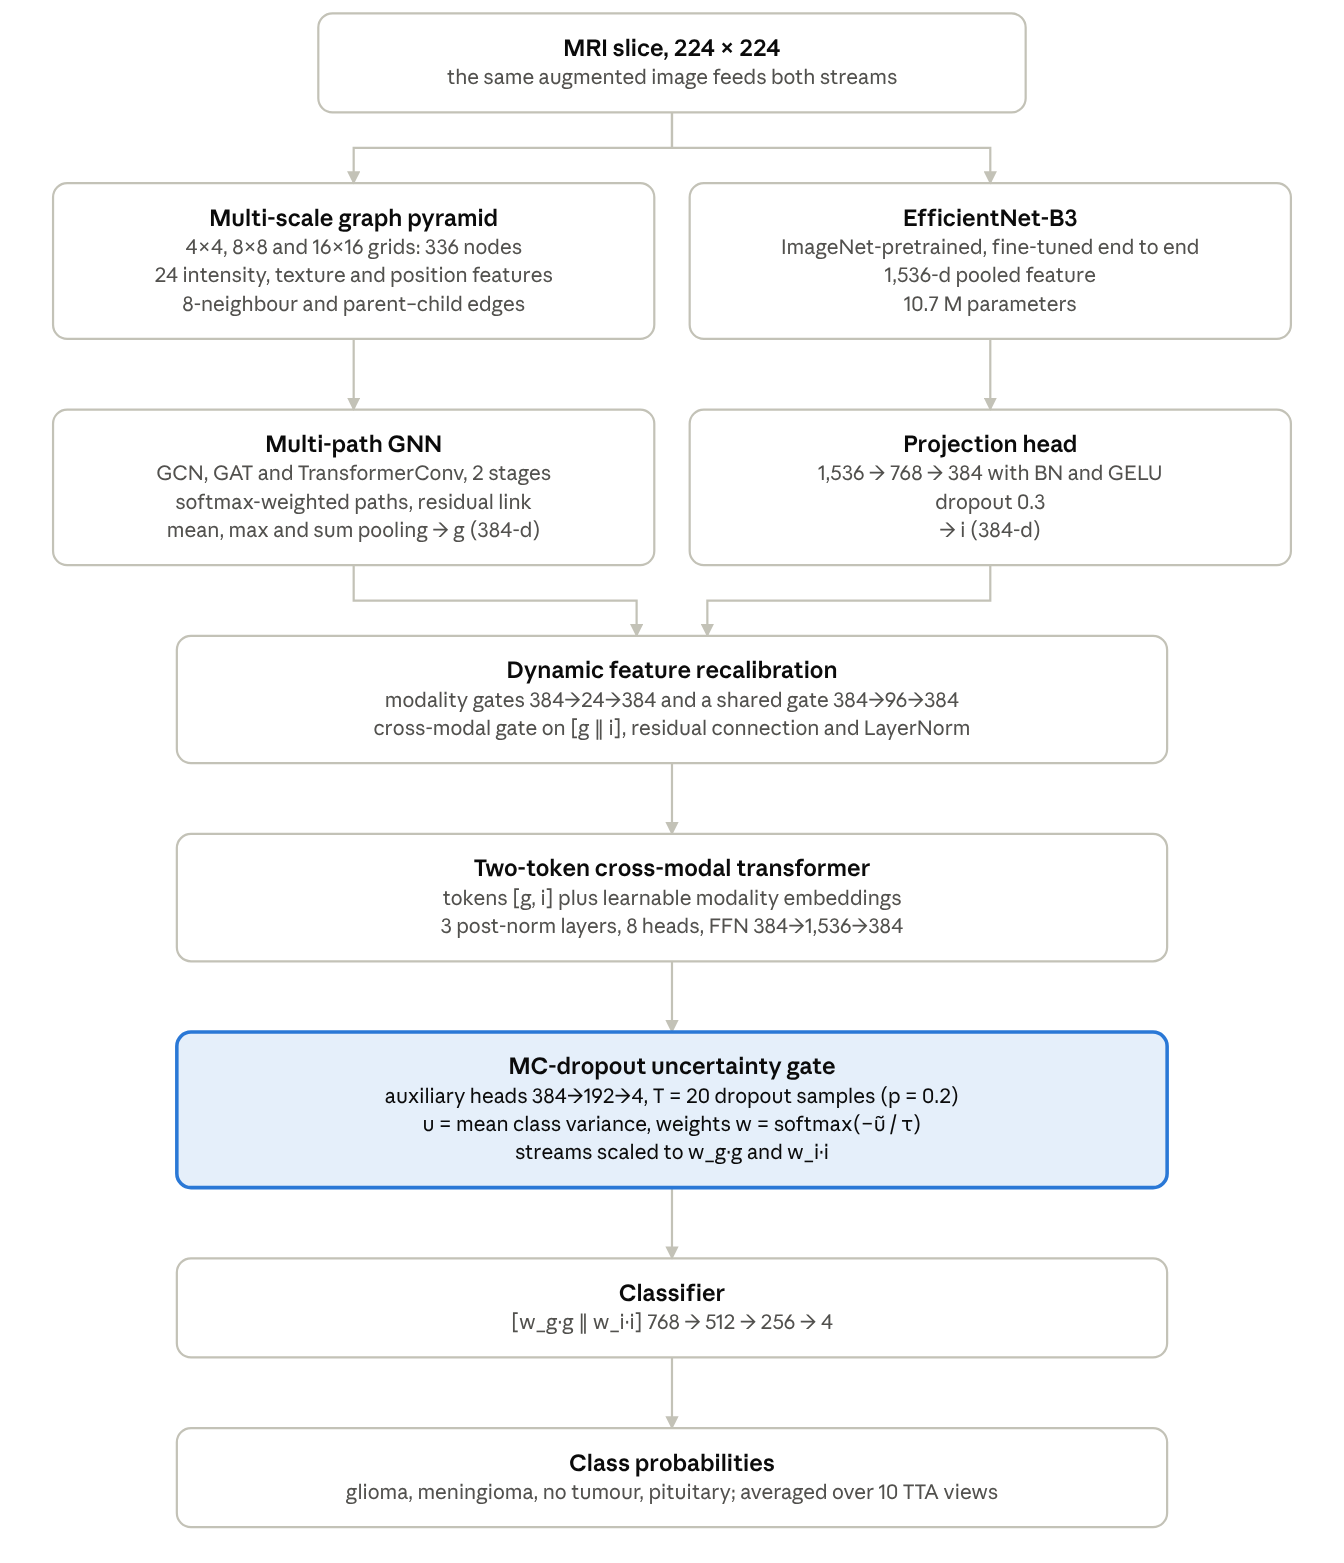
\includegraphics[width=\columnwidth]{fig2_architecture.png}
\caption{Architecture of the dual-stream classifier. Layer sizes are taken from the released code; $g$ and $i$ denote the graph and image embeddings at each stage.}
\label{fig:arch}
\end{figure}

\subsection{Input Pre-Processing}
Each image is read as three-channel RGB and resized to $224 \times 224$ pixels. The CNN input is normalised with ImageNet channel means $(0.485, 0.456, 0.406)$ and standard deviations $(0.229, 0.224, 0.225)$. Training augmentation applies a horizontal flip ($p = 0.5$) and colour jitter whose strength grows linearly over the first 15 epochs, up to brightness and contrast factors of $\pm 0.35$. The jitter also has saturation and hue terms; for slices stored as greyscale (identical channels) these leave the image unchanged, and they act only on images stored in colour. The same transformed image feeds both streams, so the two views stay spatially and photometrically aligned.

\subsection{Multi-Scale Graph Pyramid}
The greyscale image is divided into non-overlapping grids of $s \times s$ patches for $s \in \{4, 8, 16\}$, giving patches of 56, 28 and 14 pixels (Fig.~\ref{fig:pyramid}). Each patch is a node, so every image yields a graph of
\begin{equation}
N = \sum_{s \in \{4,8,16\}} s^{2} = 16 + 64 + 256 = 336 \text{ nodes.}
\end{equation}
Each node carries a 24-dimensional descriptor computed on the 0--255 intensity scale:
\begin{itemize}
\item intensity statistics: mean, standard deviation, minimum, maximum, median, variance and the 25th, 50th, 75th and 90th percentiles (intensities divided by 255, variance by $255^2$);
\item texture: mean absolute vertical and horizontal gradients and mean gradient magnitude;
\item intensity proportions: pixels above 128, below 64, above the patch mean, between 64 and 192, and above 192;
\item position and scale: the patch's grid row and column divided by $s$, their distance from $(0.5, 0.5)$, their normalised sum, $s/16$ and $1/s$.
\end{itemize}
Within each level, a node is linked to its eight spatial neighbours. Between consecutive levels, each fine node is linked in both directions to the coarse node that contains it, with parent index $(\lfloor i/2 \rfloor, \lfloor j/2 \rfloor)$. Each graph therefore has 3,004 directed edges: 2,364 within levels and 640 between them. The topology is identical for every image; only the node descriptors change.

\begin{figure*}[!t]
\centering
\figorplaceholder{fig3_graph_pyramid.png}{1.9in}{\textwidth}
\caption{Graph pyramid on one slice: the $4 \times 4$, $8 \times 8$ and $16 \times 16$ grids whose patches form the 16, 64 and 256 nodes.}
\label{fig:pyramid}
\end{figure*}

\subsection{Multi-Path Graph Neural Network}
Descriptors are projected to 128 dimensions by a linear layer, batch normalisation (BN) and GELU. Two stages follow. Each stage runs three operators in parallel on the same input: GCN~\cite{kipf2017gcn}, GAT~\cite{velickovic2018gat} and TransformerConv~\cite{shi2021masked}. The attention operators use four heads in stage~1 and two in stage~2, averaged rather than concatenated, with attention dropout 0.1. GCN and GAT add self-loops; TransformerConv does not. Each path is followed by BN and GELU, and the paths are mixed by softmax-normalised learnable weights:
\begin{align}
h^{(1)} &= \mathrm{Drop}_{0.20}\Big( \sum_{m} \alpha_m \, \mathrm{GELU}\big(\mathrm{BN}(f^{(1)}_m(x, E))\big) \Big), \\
h^{(2)} &= \mathrm{Drop}_{0.15}\Big( \mathrm{BN}\Big( h^{(1)} \nonumber \\ &\qquad + \sum_{m} \beta_m \, \mathrm{GELU}\big(\mathrm{BN}(f^{(2)}_m(h^{(1)}, E))\big) \Big) \Big),
\end{align}
where $m \in \{\mathrm{GCN}, \mathrm{GAT}, \mathrm{TR}\}$, $\alpha = \mathrm{softmax}(a)$ and $\beta = \mathrm{softmax}(b)$. The logits $a$ and $b$ start at zero, so each path initially receives a weight of $1/3$. Mean, max and sum pooling over all nodes are concatenated ($3 \times 128$; because every graph has 336 nodes, the sum-pooled vector is a fixed multiple of the mean-pooled one, and it is kept to match the trained models) and projected by a linear layer, BN, GELU and dropout (0.2) to the graph embedding $g \in \R^{384}$.

\subsection{EfficientNet-B3 Image Stream}
The image stream is the torchvision EfficientNet-B3~\cite{tan2019efficientnet} initialised with ImageNet weights, with its classifier removed. It is fine-tuned end to end, with no frozen layers, at $224 \times 224$ input rather than the $300 \times 300$ resolution used for B3 in~\cite{tan2019efficientnet}. The 1,536-dimensional pooled feature passes through a projection head: linear $1{,}536 \to 768$, BN, GELU, dropout 0.3, linear $768 \to 384$, BN, GELU. This gives the image embedding $i \in \R^{384}$.

\subsection{Dynamic Feature Recalibration}
Three kinds of sigmoid gate rescale the embeddings, in the spirit of squeeze-and-excitation~\cite{hu2018senet}. Modality gates ($384 \to 24 \to 384$ with GELU) rescale each embedding. A shared gate ($384 \to 96 \to 384$ with LayerNorm and GELU) applies to both. A cross-modal gate ($768 \to 384 \to 384$ with LayerNorm and GELU) produces one mask from the concatenated pair. With $\odot$ for element-wise multiplication and LN for layer normalisation:
\begin{align}
g_c &= g \odot \sigma\big(M_g(g)\big), & i_c &= i \odot \sigma\big(M_i(i)\big), \\
g_s &= g_c \odot \sigma\big(M_s(g_c)\big), & i_s &= i_c \odot \sigma\big(M_s(i_c)\big), \\
m &= \sigma\big(M_c([\,g_s \,\|\, i_s\,])\big), & & \\
g_r &= \mathrm{LN}(g_s \odot m + g), & i_r &= \mathrm{LN}(i_s \odot m + i).
\end{align}

\subsection{Two-Token Cross-Modal Transformer}
The recalibrated vectors are stacked as a two-token sequence $X_0 \in \R^{2 \times 384}$, and a learnable modality embedding (initialised from $\mathcal{N}(0, 0.02^2)$) is added. Three post-norm transformer blocks~\cite{vaswani2017attention} follow, each with eight-head self-attention, a feed-forward network $384 \to 1{,}536 \to 384$ with GELU, and dropout 0.05:
\begin{align}
\tilde{X}_l &= \mathrm{LN}\big(X_{l-1} + \mathrm{MHA}(X_{l-1}, X_{l-1}, X_{l-1})\big), \\
X_l &= \mathrm{LN}\big(\tilde{X}_l + \mathrm{FFN}(\tilde{X}_l)\big).
\end{align}
The first output token is the refined graph vector $z_g$ and the second the refined image vector $z_i$. With two tokens, each head's attention is a $2 \times 2$ weighting between the modalities.

\subsection{MC-Dropout Uncertainty-Guided Gating}
Each modality has an auxiliary head $H_m$ ($384 \to 192 \to 4$ with GELU). To estimate how stable each head's prediction is, the embedding is replicated $T = 20$ times and passed through dropout with $p = 0.20$, which stays active at inference. The per-modality uncertainty is the class-averaged variance of the sampled probabilities~\cite{gal2016dropout}:
\begin{align}
p_m^{(t)} &= \mathrm{softmax}\big(H_m(\mathrm{Drop}_{0.2}(z_m))\big), \\
u_m &= \frac{1}{C} \sum_{c=1}^{C} \mathrm{Var}_{t=1,\dots,T}\big(p^{(t)}_{m,c}\big), \qquad C = 4.
\end{align}
The two scores are normalised by their mean and turned into fusion weights by a softmax with a learnable temperature $\tau = \mathrm{softplus}(\rho) + 10^{-6}$, where $\rho$ is initialised at 0 (so $\tau$ starts at 0.693):
\begin{align}
\tilde{u}_m &= \frac{u_m}{\tfrac{1}{2}(u_g + u_i) + 10^{-8}}, \\
[w_g, w_i] &= \mathrm{softmax}\big(-[\tilde{u}_g, \tilde{u}_i]/\tau\big).
\end{align}
The weighted vectors $w_g z_g$ and $w_i z_i$ are passed on. Dropout is applied only in front of the auxiliary heads, so $u_m$ measures the stability of those heads rather than the full epistemic uncertainty of the network. Gradients flow through the uncertainty computation; it is not detached.

\subsection{Classification Head and Objective}\label{sec:loss}
The concatenated vector $[w_g z_g \,\|\, w_i z_i] \in \R^{768}$ passes through linear $768 \to 512$, BN, GELU, dropout 0.4, linear $512 \to 256$, BN, GELU, dropout 0.3 and linear $256 \to 4$. The loss combines the main cross-entropy with the two auxiliary heads (applied to the non-dropped embeddings). All three terms use label smoothing $\varepsilon = 0.03$~\cite{szegedy2016inception} on logits clipped to $[-20, 20]$:
\begin{equation}
\mathcal{L} = \mathcal{L}_{\mathrm{main}} + \lambda \cdot \tfrac{1}{2}\big(\mathcal{L}_{g} + \mathcal{L}_{i}\big), \qquad \lambda = 0.15.
\end{equation}

\subsection{Test-Time Augmentation}\label{sec:tta}
At test time, class probabilities are averaged over ten deterministic views~\cite{wang2019tta}: identity, horizontal flip, rotations of $\pm 5^\circ$, brightness $\times 0.9$ and $\times 1.1$, contrast $\times 0.9$ and $\times 1.1$, saturation $\times 1.1$, and horizontal flip with brightness $\times 1.1$. Each view feeds both streams:
\begin{equation}
p_{\mathrm{final}}(x) = \frac{1}{10} \sum_{a=1}^{10} \mathrm{softmax}\big(f(T_a(x))\big).
\end{equation}
For slices stored as greyscale, the saturation view equals the identity view, so for those images the ensemble effectively contains nine distinct views, with the original image counted twice. The TTA views are resized with the image library's default filter, whereas training uses bilinear resizing; this small preprocessing difference is reported for reproducibility.

% =====================================================================
\section{Experimental Setup and Evaluation Protocol}
\subsection{Implementation}
The model was implemented in PyTorch~\cite{paszke2019pytorch} with PyTorch Geometric~\cite{fey2019pyg} and the torchvision EfficientNet-B3. It was trained on single-GPU Kaggle notebook sessions (\todo{GPU model}; PyTorch \todo{version}, PyTorch Geometric \todo{version}) with automatic mixed precision. Each fold ran as a separate session, with only the fold index changed.

\subsection{Cross-Validation and Test Isolation}\label{sec:cv}
Stratified five-fold cross-validation (shuffled, random state 42) was applied to the merged 12,064 images, giving test folds of 2,412--2,413 images with the class proportions of Table~\ref{tab:classes}. Within the remaining 80\% of each fold, a stratified 8\% subset (random state $42 + k$ for zero-based fold $k$) served for validation and checkpoint selection. On a whole-dataset basis, each fold used 73.6\% of images for training, 6.4\% for validation and 20\% for testing. Test images were used only after the fold's checkpoint had been selected and reloaded.

The split is at image level. Patient identifiers are unavailable, so patient-level independence cannot be enforced, and the augmented copies described in Section~\ref{sec:data} can fall on both sides of a split. Section~\ref{sec:leak} quantifies this.

\subsection{Optimisation and Model Selection}
The training configuration, identical for all folds, is listed in Table~\ref{tab:config}. The checkpoint with the highest validation accuracy was kept. Because the MC dropout in the gate also runs during validation, validation accuracy is itself a slightly stochastic estimate. We return to this in Section~\ref{sec:calib}.

\begin{table}[!t]
\caption{Training Configuration, Identical for All Folds}
\label{tab:config}
\centering
\footnotesize
\begin{tabular}{@{}>{\raggedright\arraybackslash}p{2.35cm}>{\raggedright\arraybackslash}p{6.0cm}@{}}
\toprule
Setting & Value \\
\midrule
Optimiser & AdamW~\cite{loshchilov2019adamw}, weight decay 0.01 \\
Peak learning rate & $3 \times 10^{-4}$; $6 \times 10^{-5}$ for GAT, TransformerConv and cross-modal attention modules (with their normalisation layers) \\
Schedule & OneCycle~\cite{smith2019superconvergence} over 30 epochs, 10\% warm-up, cosine annealing \\
Batch size & 36 (247 training batches per epoch) \\
Max.\ epochs / early stopping & 30 / patience 5 on validation accuracy \\
Loss & Section~\ref{sec:loss}: label smoothing 0.03, auxiliary weight $\lambda = 0.15$ \\
Gradient clipping & global norm 1.0 \\
MC-dropout samples / rate & $T = 20$ / $p = 0.20$ \\
Test-time augmentation & 10 deterministic views (Section~\ref{sec:tta}) \\
Random seed & 42 (Python, NumPy, PyTorch, CUDA; deterministic cuDNN) \\
\bottomrule
\end{tabular}
\end{table}

\subsection{Metrics}
We report accuracy and macro-averaged precision, recall and F1, which weight the four classes equally. With $N$ test images, $C = 4$ classes and per-class precision $P_c$ and recall $R_c$:
\begin{equation}
\mathrm{Acc} = \frac{1}{N}\sum_{n=1}^{N} \mathbf{1}[\hat{y}_n = y_n], \qquad \mathrm{F1}_{\mathrm{macro}} = \frac{1}{C}\sum_{c=1}^{C} \frac{2 P_c R_c}{P_c + R_c}.
\end{equation}
Class-wise sensitivity (recall) and specificity are computed one-vs-rest. Calibration is measured by top-label ECE with ten equal-width confidence bins $B_b$~\cite{guo2017calibration,naeini2015bbq} and by the multiclass Brier score~\cite{brier1950verification}, summed over classes (range 0--2):
\begin{align}
\mathrm{ECE} &= \sum_{b=1}^{10} \frac{|B_b|}{N}\,\big|\mathrm{acc}(B_b) - \mathrm{conf}(B_b)\big|, \\
\mathrm{Brier} &= \frac{1}{N}\sum_{n=1}^{N}\sum_{c=1}^{C}\big(p_{n,c} - \mathbf{1}[y_n = c]\big)^2.
\end{align}
We also report the negative log-likelihood (NLL) of the true class.

\subsection{Aggregation and Verification}
Fold-level metrics are summarised as mean $\pm$ sample standard deviation ($n = 5$). Each image is predicted only by the model of the fold in which it was held out. The five prediction files were therefore concatenated into one set of 12,064 out-of-fold (OOF) predictions, used for the pooled confusion matrix, per-class analysis and reliability diagram. The five models are never ensembled on these data. Pooled 95\% confidence intervals come from 2,000 bootstrap resamples~\cite{efron1993bootstrap}, both over images and over clusters of augmented copies of the same slice.

Before analysis, every saved metric was recomputed independently from the per-image predictions. The five test folds were checked to be pairwise disjoint and to cover all 12,064 images exactly once. All recomputed values matched the saved ones (absolute differences below $10^{-11}$).

% =====================================================================
\section{Results}\label{sec:results}
\subsection{Fold-Wise Performance}
Across the five folds, accuracy was $99.15 \pm 0.39\%$ and macro-F1 $99.15 \pm 0.40\%$ (Table~\ref{tab:folds}). Folds 1--4 lay within 99.25--99.46\%. Fold~5 reached 98.47\%, with 37 errors against 13--18 in the other folds.

\begin{table*}[!t]
\caption{Held-Out Performance per Fold (Macro-Averaged Precision, Recall and F1)}
\label{tab:folds}
\centering
\footnotesize
\setlength{\tabcolsep}{3pt}
\begin{tabular}{@{}crccccccccr@{}}
\toprule
Fold & Images & Accuracy (\%) & Precision (\%) & Recall (\%) & F1 (\%) & ECE & Brier & NLL & Errors \\
\midrule
1 & 2,413 & 99.30 & 99.26 & 99.38 & 99.32 & 0.0187 & 0.0132 & 0.0460 & 17 \\
2 & 2,413 & 99.25 & 99.28 & 99.23 & 99.25 & 0.0190 & 0.0121 & 0.0434 & 18 \\
3 & 2,413 & 99.25 & 99.28 & 99.23 & 99.25 & 0.0188 & 0.0132 & 0.0467 & 18 \\
4 & 2,413 & 99.46 & 99.46 & 99.46 & 99.46 & 0.0231 & 0.0091 & 0.0406 & 13 \\
5 & 2,412 & 98.47 & 98.40 & 98.49 & 98.44 & 0.0248 & 0.0256 & 0.0696 & 37 \\
\midrule
\textbf{Mean $\pm$ SD} & -- & $\mathbf{99.15 \pm 0.39}$ & $\mathbf{99.14 \pm 0.42}$ & $\mathbf{99.16 \pm 0.39}$ & $\mathbf{99.15 \pm 0.40}$ & $\mathbf{0.021 \pm 0.003}$ & $\mathbf{0.015 \pm 0.006}$ & $\mathbf{0.049 \pm 0.012}$ & 103 \\
\bottomrule
\end{tabular}
\end{table*}

\subsection{Pooled Out-of-Fold Performance}
Pooling the 12,064 out-of-fold predictions gave 11,961 correct classifications: 99.15\% accuracy (95\% CI 98.99--99.31\%) and macro-F1 99.15\% (98.98--99.31\%). Resampling whole clusters of augmented copies instead of single images widened the intervals by at most 0.02 percentage points (accuracy 98.97--99.32\%). Pooled ECE was 0.020 (0.019--0.022), Brier 0.015 (0.012--0.017) and NLL 0.049.

\subsection{Per-Class Performance and Errors}
All four classes exceeded 98.5\% sensitivity and 99.6\% specificity (Table~\ref{tab:perclass}). Pituitary tumours and tumour-free scans were recognised best; meningioma was hardest.

\begin{table}[!t]
\caption{Per-Class Results on the Pooled Out-of-Fold Predictions ($n = 12{,}064$)}
\label{tab:perclass}
\centering
\footnotesize
\setlength{\tabcolsep}{4pt}
\begin{tabular}{@{}lrcccc@{}}
\toprule
Class & Support & Prec. (\%) & Sens. (\%) & Spec. (\%) & F1 (\%) \\
\midrule
Glioma & 3,773 & 99.33 & 98.97 & 99.70 & 99.15 \\
Meningioma & 2,729 & 98.90 & 98.53 & 99.68 & 98.72 \\
No tumour & 2,432 & 99.22 & 99.55 & 99.80 & 99.38 \\
Pituitary & 3,130 & 99.08 & 99.58 & 99.68 & 99.33 \\
\bottomrule
\end{tabular}
\end{table}

The 103 errors concentrate between tumour types (Fig.~\ref{fig:confusion}). Glioma--meningioma confusions account for 43 (42\%), meningioma--pituitary for 22 and glioma--pituitary for 8. Nineteen of 9,632 tumour images (0.20\%) were called tumour-free, and 11 of 2,432 tumour-free images (0.45\%) were called tumour.

\begin{figure}[!t]
\centering
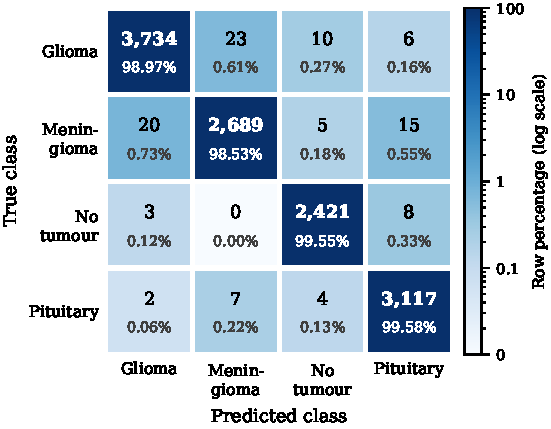
\includegraphics[width=\columnwidth]{fig_confusion.pdf}
\caption{Pooled out-of-fold confusion matrix of folds 1--5 ($n = 12{,}064$). Each cell gives the image count and the row percentage; shading follows the row percentage on a logarithmic scale so that small error counts remain visible.}
\label{fig:confusion}
\end{figure}

\subsection{Calibration}
The model is well calibrated below 0.9 confidence and slightly under-confident above it (Fig.~\ref{fig:reliability}). In the top bin, which holds 11,803 images (97.8\%), accuracy was 99.64\% while mean confidence was 97.66\%; this gap accounts for almost all of the ECE. The highest probability assigned to any image was 0.988.

\begin{figure}[!t]
\centering
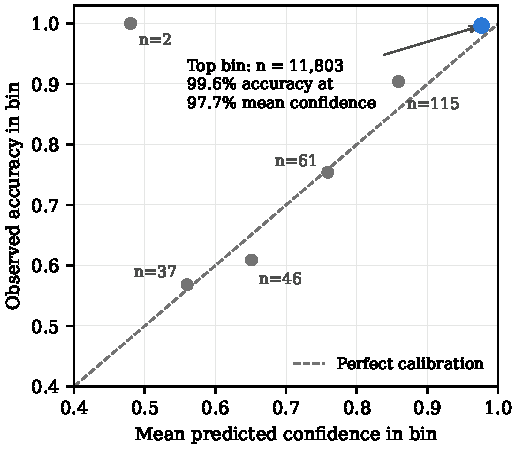
\includegraphics[width=\columnwidth]{fig4_reliability.pdf}
\caption{Reliability diagram of the pooled out-of-fold predictions of folds 1--5 (12,064 images).}
\label{fig:reliability}
\end{figure}

Confidence is informative for triage. The 261 images (2.2\%) predicted with confidence below 0.9 had 77.0\% accuracy and contained 60 of the 103 errors (58\%). However, 29 errors (28\%) were made at confidence of 0.95 or higher, so low confidence does not flag every error.

\subsection{Model Size and Cost}
The model has 19,350,155 trainable parameters (Table~\ref{tab:params}). A single forward pass costs about 2.25 GFLOPs of dense operations, measured with the PyTorch FLOP counter (\texttt{torch.utils.flop\_counter}) at $224 \times 224$ input; graph message passing is not included.

\begin{table}[!t]
\caption{Parameter Count per Module (Identical in All Five Checkpoints)}
\label{tab:params}
\centering
\footnotesize
\begin{tabular}{@{}lrr@{}}
\toprule
Module & Parameters & Share \\
\midrule
EfficientNet-B3 features & 10,696,232 & 55.3\% \\
Image projection head & 1,478,016 & 7.6\% \\
Cross-modal transformer & 5,324,160 & 27.5\% \\
Multi-path GNN (graph stream) & 617,222 & 3.2\% \\
Dynamic recalibration & 557,520 & 2.9\% \\
Classifier & 527,620 & 2.7\% \\
Uncertainty heads and $\tau$ & 149,385 & 0.8\% \\
\midrule
\textbf{Total} & \textbf{19,350,155} & \textbf{100\%} \\
\bottomrule
\end{tabular}
\end{table}

On a four-core Intel Xeon virtual machine (2.8\,GHz), one forward pass took about 84\,ms and building one graph took about 156\,ms. Graph construction therefore dominates CPU inference, and with ten TTA views it is repeated ten times per image. GPU latency was not measured.

\subsection{Learned Fusion Parameters}\label{sec:learned}
The learned path weights stayed close to their initial value of $1/3$. In fold~1, $\mathrm{softmax}(a) = (0.328, 0.333, 0.339)$ and $\mathrm{softmax}(b) = (0.333, 0.337, 0.330)$ for (GCN, GAT, TransformerConv). Fold~2 gave $(0.331, 0.334, 0.335)$ and $(0.333, 0.337, 0.331)$. The gate temperature rose from its initial 0.693 to 0.764 (fold~1) and 0.773 (fold~2). Folds 3--5 were not inspected for these values.

% =====================================================================
\section{Discussion}
\subsection{Does Duplicate Leakage Inflate Accuracy?}\label{sec:leak}
Augmented copies crossed the split for almost every affected image, yet they were classified no better than the rest (Table~\ref{tab:leak}). We call a test image \textit{leaked} when another copy of the same source slice was among the test images of a different fold, and therefore in this fold's training data. Pooled over folds, 4,238 of the 4,246 augmented-family images (99.8\%) were leaked. Their accuracy was 99.15\%, against 99.14\% for the other 7,826 images. Per-fold differences went in both directions, consistent with noise.

\begin{table}[!t]
\caption{Accuracy of Test Images Whose Source Slice Was Also in the Training Partition (Leaked), Versus All Other Test Images}
\label{tab:leak}
\centering
\footnotesize
\setlength{\tabcolsep}{3.5pt}
\begin{tabular}{@{}crrcc@{}}
\toprule
Fold & \shortstack{Augmented-\\family images} & \shortstack{Leaked (copy\\in training)} & \shortstack{Acc., leaked\\(\%)} & \shortstack{Acc., other\\images (\%)} \\
\midrule
1 & 856 & 853 (99.6\%) & 98.83 & 99.55 \\
2 & 832 & 831 (99.9\%) & 99.52 & 99.12 \\
3 & 833 & 831 (99.8\%) & 99.28 & 99.24 \\
4 & 853 & 852 (99.9\%) & 99.65 & 99.36 \\
5 & 872 & 871 (99.9\%) & 98.51 & 98.44 \\
\midrule
\textbf{Pooled} & \textbf{4,246} & \textbf{4,238 (99.8\%)} & \textbf{99.15} & \textbf{99.14} \\
\bottomrule
\end{tabular}
\end{table}

This comparison bounds only the leakage that file names reveal. Grouping copies by file name reduces the 12,064 images to 8,438 clusters, whereas the de-duplicated Version~7 of the dataset retains 5,941 images~\cite{bdneuro2025v7}. Up to about 2,500 further near-duplicates, probably mostly across source collections, may therefore be invisible to our grouping. The ``other images'' in Table~\ref{tab:leak} are not proven leak-free. Our figures should be read as image-level estimates, and a duplicate-aware (grouped) split is the definitive test.

\subsection{Where the Errors Come From}
Error rates differ markedly by data source (Table~\ref{tab:errfam}). The 249 images named \fname{image(n)}, the test-split naming of one public source~\cite{bhuvaji2020kaggle}, have a 6.0\% error rate, seven times the average of 0.85\%. Users of a public mirror of a related compilation have reported mislabelled glioma images in this source~\cite{chaki2023dataport}. Thirteen of these 15 errors are gliomas predicted as meningioma or tumour-free, nine of them with confidence of 0.95 or more. This points to label noise rather than model failure. Expert re-reading of these images is needed to confirm this.

\begin{table}[!t]
\caption{Error Rate by File-Name Family (Pooled Out-of-Fold Predictions)}
\label{tab:errfam}
\centering
\footnotesize
\begin{tabular}{@{}lrrr@{}}
\toprule
File-name family & Images & Errors & Error rate (\%) \\
\midrule
\fname{image(n)} & 249 & 15 & 6.02 \\
\fname{N\#}, \fname{\# no} & 76 & 1 & 1.32 \\
\fname{Tr-xx\_\#\#\#\#} & 3,784 & 37 & 0.98 \\
\fname{G/M/P/N\_\#\#\#} (+ augmentations) & 4,246 & 36 & 0.85 \\
\fname{gg/m/p (n)} & 935 & 6 & 0.64 \\
\fname{\#.jpg} & 1,914 & 6 & 0.31 \\
\fname{Te-xx\_\#\#\#\#} & 858 & 2 & 0.23 \\
\bottomrule
\end{tabular}
\end{table}

A second cluster consists of nine \fname{Tr-me\_*} meningiomas predicted as pituitary tumours with confidence 0.95--0.98 (the most confident errors are shown in Fig.~\ref{fig:errors}). Three have near-consecutive identifiers (0828, 0829, 0831) and may be neighbouring slices of one patient. Meningiomas near the sella can resemble pituitary adenomas, so these cases may reflect genuine diagnostic difficulty. Errors also cluster within source slices: for four slices, two copies of the same slice were misclassified together (one slice in fold~1, one in fold~3 and two in fold~5). Errors are therefore not independent, and image-level confidence intervals are somewhat optimistic.

\begin{figure*}[!t]
\centering
\figorplaceholder{fig5_confident_errors.png}{3.0in}{\textwidth}
\caption{The eight most confident out-of-fold errors, each shown with its file-name family, true label, predicted label and confidence.}
\label{fig:errors}
\end{figure*}

\subsection{Calibration and Fold-to-Fold Variability}\label{sec:calib}
The residual miscalibration is a ceiling effect of label smoothing. With $\varepsilon = 0.03$ and four classes, the training target for the true class is $1 - \varepsilon + \varepsilon/4 = 0.9775$. Training pulls the predicted probability of the true class towards this target rather than towards 1; accordingly, mean confidence in the top bin is 97.66\% (maximum 0.988), while top-bin accuracy is 99.64\%. Label smoothing is known to produce such conservative confidence~\cite{muller2019labelsmoothing}. The ECE we report therefore reflects the loss design, not the uncertainty gate, whose contribution to calibration this study does not isolate. Post-hoc temperature scaling fitted on the validation split~\cite{guo2017calibration} would probably remove most of the gap.

Fold~5 was the only weak fold. It produced 140 predictions below 0.9 confidence, against 19--40 in the other folds, and its errors rose in all major data sources and in both original folders. This pattern points to a weaker trained model rather than a harder test fold. A plausible cause is checkpoint selection on validation accuracy: on about 770 validation images near 99\% accuracy, successive epochs differ by one or two images, and the gate's MC dropout adds sampling noise. Selecting on validation loss with fixed dropout seeds would remove this source of variability.

\subsection{What the Trained Parameters Reveal}\label{sec:params}
The parameter analysis tempers the architectural claims. The graph stream holds 3.2\% of the parameters, while the two-token cross-modal transformer holds 27.5\%; with two tokens, each attention head reduces to a $2 \times 2$ weighting of the modalities. The learnable path weights of the multi-path GNN stayed within 0.006 of $1/3$ in both inspected folds, so the three operators act as an equal-weight average rather than an adaptively selected mixture. The gate temperature moved only slightly from its initial value.

None of this shows that the components are useless. It does show that their individual contributions are not established by the present experiments. Component ablations under the same folds are required: image-only, graph-only, concatenation, fixed 0.5/0.5 gate, transformer replaced by a multilayer perceptron, and a single GNN operator.

\subsection{Relation to Prior Results}
Published accuracies are not directly comparable to ours. Tummala \textit{et al.} reported 98.7\% with a ViT ensemble on the three-class figshare data~\cite{tummala2022classification}, and G\"{u}rsoy and Kaya 93.68\% with a CNN--GCN hybrid on a 10,847-image collection~\cite{gursoy2024braingcn}. Datasets, class sets and split units differ across these studies, and duplication levels are rarely reported. We therefore make no state-of-the-art claim. A fair comparison requires retraining baselines under identical, duplicate-aware folds.

% =====================================================================
\section{Limitations and Future Work}
\begin{enumerate}
\item \textit{Image-level splitting:} Patient identifiers are unavailable, and cross-source near-duplicates beyond the file-name groups could not be excluded. The reported accuracy is therefore an image-level estimate, not evidence of generalisation to unseen patients. Next step: grouped five-fold cross-validation with groups formed from file-name stems and perceptual-hash near-duplicates, and a parallel analysis on the de-duplicated Version~7~\cite{bdneuro2025v7}.
\item \textit{No component ablations or retrained baselines:} The contribution of the graph stream, recalibration, transformer and uncertainty gate is not isolated (Section~\ref{sec:params}), and no baseline was retrained under the same folds. Next step: the ablation set of Section~\ref{sec:params} and three to four standard CNN and transformer baselines on identical folds, compared by McNemar's test on out-of-fold predictions.
\item \textit{Single dataset, no external test:} All images come from one compiled collection, part of which overlaps by naming with other public sets. An independent test set must first be checked for overlap with the training data.
\item \textit{Provenance and label quality:} The origin of the images was inferred from file names and not verified by image matching. One source shows a raised error rate consistent with label noise. Expert re-reading of the 103 misclassified images would separate label noise from model error.
\item \textit{Single seed and stochastic selection:} Each fold was trained once (seed 42), and checkpoints were selected on a stochastic, saturated validation accuracy (Section~\ref{sec:calib}). Development was iterative: an earlier configuration was evaluated on fold~1 before the final design was fixed, so fold~1 was not strictly untouched during development.
\item \textit{Two-dimensional slices:} The model sees single 2D slices and ignores volumetric context and other MRI sequences.
\item \textit{Inference cost:} GPU latency was not measured. Graph construction on the CPU dominates inference time when repeated for ten TTA views.
\item \textit{Not a clinical device:} The model has not been evaluated prospectively or against radiologists, and its outputs are not diagnoses.
\end{enumerate}

% =====================================================================
\section{Conclusion}
A dual-stream EfficientNet-B3 and multi-scale graph model with uncertainty-gated fusion classified four-class brain tumour MRI with $99.15 \pm 0.39\%$ accuracy and $99.15 \pm 0.40\%$ macro-F1 under image-level stratified five-fold cross-validation (RQ1). Sensitivity was at least 98.5\% and specificity at least 99.7\% for every class, and only 0.20\% of tumour images were called tumour-free. The probability estimates were slightly conservative, with an ECE of 0.021 that stems mainly from label smoothing, and confidence below 0.9 flagged 58\% of all errors in 2.2\% of images (RQ2). More than a third of the dataset consists of augmented copies of 620 slices whose siblings sat in training, yet their accuracy did not differ from that of the remaining images (RQ3).

These results are image-level estimates on one compiled dataset. The near-uniform path weights and the parameter distribution show that the value of each architectural component remains to be demonstrated. Grouped, duplicate-aware validation, component ablations, retrained baselines and an independent external test are the necessary next steps before any claim of clinical generalisation.

% =====================================================================
\section*{Data and Code Availability}
The dataset is publicly available on Mendeley Data, Version~1 (doi:10.17632/zwr4ntf94j.1), under a CC~BY~4.0 licence~\cite{hira2025mendeley}. The unmodified copy used for training is mirrored at \url{https://www.kaggle.com/datasets/arafatrahmann/my-data221}. The training script, the fold assignments, the per-image out-of-fold predictions and the audit scripts are available at \todo{repository URL}.

\section*{Ethics Statement}
This study used only a public, de-identified dataset. No new data were collected and no ethics approval was required.

\section*{Acknowledgment}
\todo{To be completed. Author contributions (e.g.\ CRediT roles) and any use of AI-assisted tools in analysis or writing should be stated as required by the target journal.}

\bibliographystyle{IEEEtran}
\bibliography{references}

\end{document}
